\cleardoublepage
\pagestyle{fancy} % Kopf- und Fußzeilen aktivieren (=> Paket "fancyhdr")
\fancyhead{}
\fancyhf{}
\renewcommand{\headrulewidth}{0pt}
\renewcommand{\footrulewidth}{0.4pt}
\fancyfoot[L]{AMS Project - Report}
\fancyfoot[R] {Page \thepage}
\pagenumbering{arabic}

\section{Introduction}

This research project has the objective to design a system that is able to navigate on its own in an unknown environment, search and identify an object\footnote{The action of searching and identifying an object will further be referenced as object hunt.} and build a map of the navigated route as well as a map of its surroundings. The system as a whole will consist of a mobile device, further named robot, and an auxiliary external computer. As the robot on its own only offers limited computing power, it will outsource computing intensive tasks to the external computer. Hence multiple processes on different platforms will be involved. To be able to operate in any arbitrary location, the system shall be independent of any additional hardware as for example networking devices. Besides it is desirable to design the system in such a manner, that supplementary software, which is not planned now, can be added easily by additional external computers. Figure \ref{fig:connection} shows a potential connection between the robot, i.e. the symbol in the middle, and other devices via a wireless LAN\footnote{A LAN (local area network) is a computer network that interconnects computers within a limited area.}.

\begin{figure}[H]
\centering
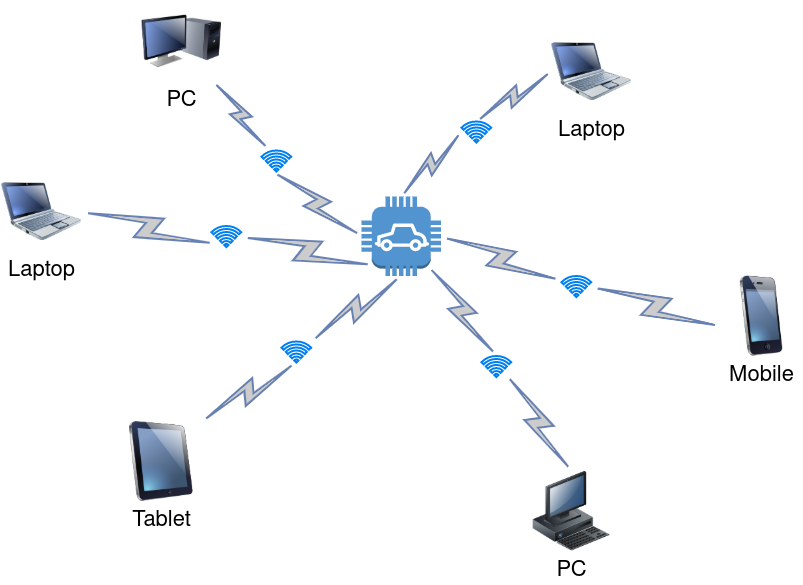
\includegraphics[scale=0.45]{sources/connection_overview.png}
\caption[Display of possible connections]{Display of possible connections}
\label{fig:connection}
\end{figure}

The robot will steer by controlling multiple motors, which will be attached to wheels. Furthermore it will be able to capture its surroundings and any obstacle near it by distance measurement sensors. They will be mounted around the robot in order to register surroundings in any direction. Additional sensors will keep track of the orientation in space and movements of the robot. The target object will be identified by processing data of a visual sensor, i.e. a camera attached to the robot.

The aim of the robot is to avoid collisions in any environment and find the target object. When the target object is found it shall stop navigating and indicate the successful identification of the object to the user.


%Therefore the mobile system needs to be able to handle connections to external processes dynamically and independent of the current state or other events. The absence of an external process will result in loss of the regarding function, any other functionality shall be available regardless. This allows a flexible and modular software structure, where further processes can be added without disturbing the fundamental functionality.


